% Implements a drawing of the "Rule of Sarrus"
% https://en.wikipedia.org/wiki/Rule_of_Sarrus
% Based on code by Thorsten Donig on 
% https://tex.stackexchange.com/a/32981
% Renders on https://www.papeeria.com/

\documentclass{minimal}
\usepackage{tikz}
\usetikzlibrary{calc,matrix}

\begin{document}
  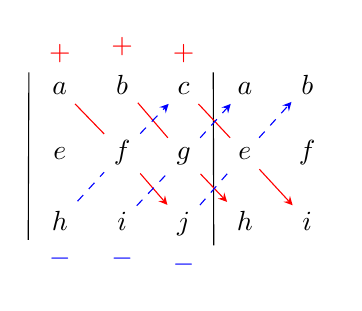
\begin{tikzpicture}[>=stealth]
    \matrix [%
      matrix of math nodes,
      column sep=1em,
      row sep=1em
    ] (sarrus) {%
      a & b & c & a & b \\
      e & f & g & e & f \\
      h & i & j & h & i \\
    };

    \path ($(sarrus-1-1.north west)-(0.5em,0)$) edge ($(sarrus-3-1.south west)-(0.5em,0)$)
          ($(sarrus-1-3.north east)+(0.5em,0)$) edge ($(sarrus-3-3.south east)+(0.5em,0)$)
          (sarrus-1-1)                          edge[red]            (sarrus-2-2)
          (sarrus-2-2)                          edge[->,red]         (sarrus-3-3)
          (sarrus-1-2)                          edge[red]            (sarrus-2-3)
          (sarrus-2-3)                          edge[->,red]         (sarrus-3-4)
          (sarrus-1-3)                          edge[red]            (sarrus-2-4)
          (sarrus-2-4)                          edge[->,red]         (sarrus-3-5)
          (sarrus-3-1)                          edge[dashed,blue]    (sarrus-2-2)
          (sarrus-2-2)                          edge[->,dashed,blue] (sarrus-1-3)
          (sarrus-3-2)                          edge[dashed,blue]    (sarrus-2-3)
          (sarrus-2-3)                          edge[->,dashed,blue] (sarrus-1-4)
          (sarrus-3-3)                          edge[dashed,blue]    (sarrus-2-4)
          (sarrus-2-4)                          edge[->,dashed,blue] (sarrus-1-5);

    \foreach \c in {1,2,3} {\node[anchor=south,red] at (sarrus-1-\c.north) {$+$};};
    \foreach \c in {1,2,3} {\node[anchor=north,blue] at (sarrus-3-\c.south) {$-$};};
  \end{tikzpicture}
\end{document}
